\section{Capire il ritardo di input}
Per capire perché il ritardo di input esiste, è necessario conoscere tutti i fattori coinvolti, dalla pressione del tasto fino al cambio di colore dei pixel sullo schermo, e come il sistema e le applicazioni reagiscono all'input. Questa sezione prende come riferimento la pressione di un tasto su un mouse USB cablato, che è lo scenario più comune e d'interesse, ma considerazioni analoghe si applicano anche a controller dedicati, tastiere, eccetera.

La figura \ref{fig:nvidia_latencypipeline} presa dalla documentazione di Nvidia Reflex mostra, seppur esagerando leggermente alcuni tempi poiché è materiale di marketing, tutti i contributori alla latenza del sistema. In questa sezione saranno discussi individualmente.

\begin{figure}[h]
	\centering
	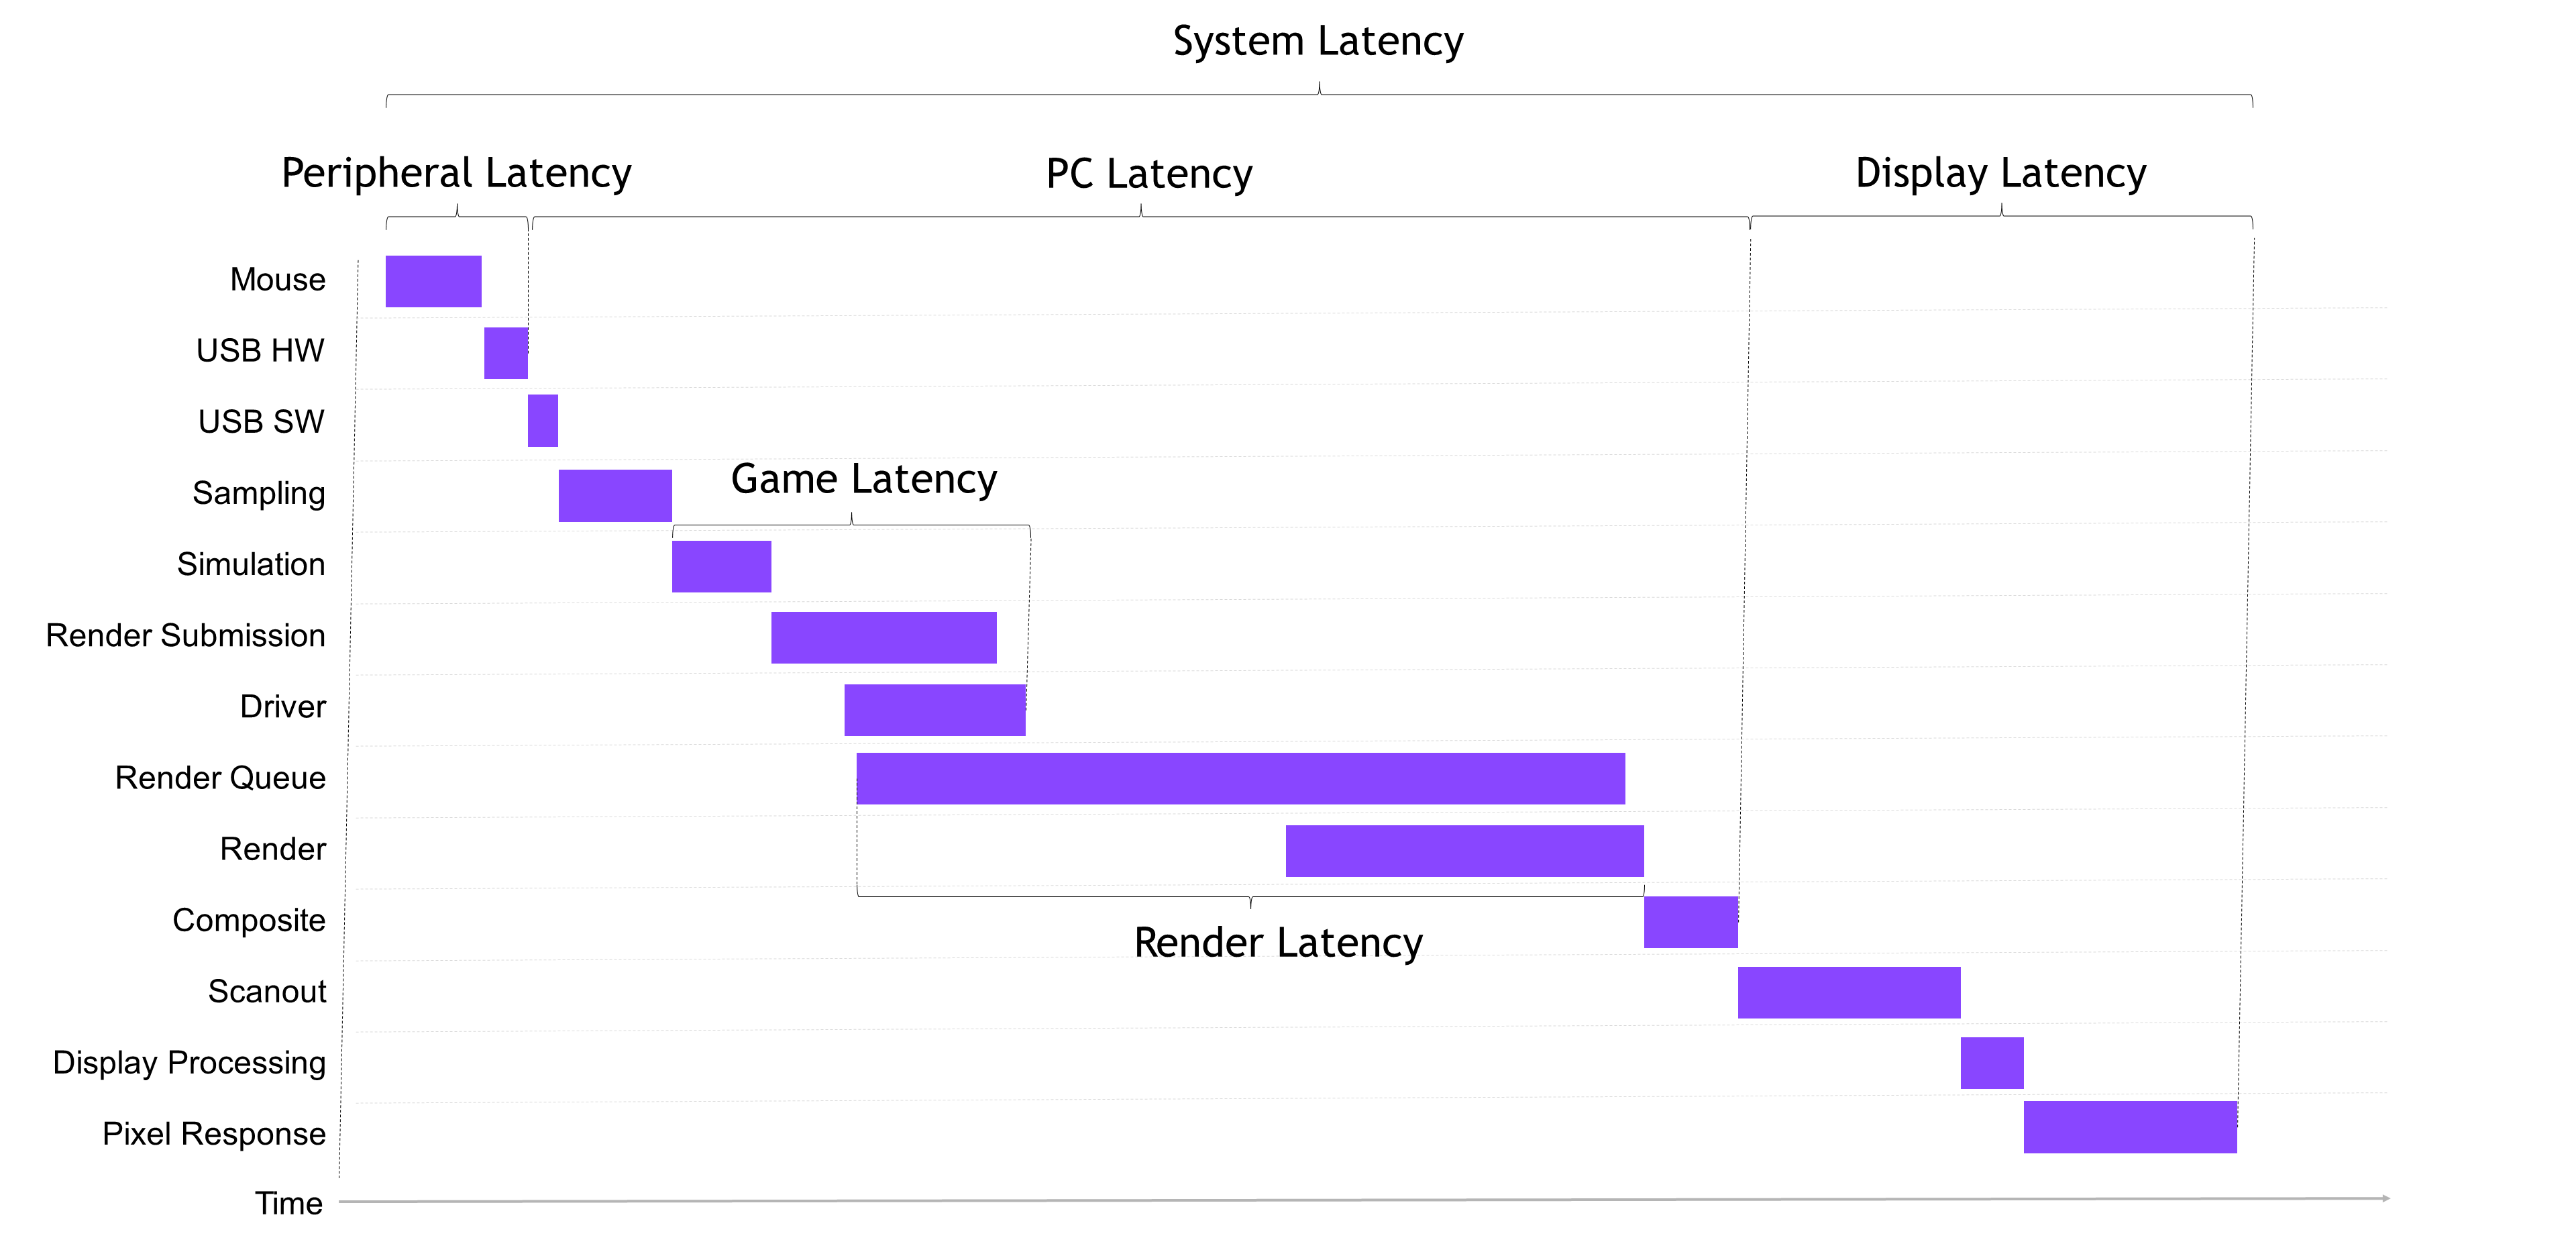
\includegraphics[width=\textwidth]{Chapter01/res/nvidia_latencypipeline.png}
	\caption{Componenti della latenza (dalla documentazione di Nvidia Reflex, 2020)}
	\label{fig:nvidia_latencypipeline}
\end{figure}

Nel momento in cui l'utente preme un pulsante sul mouse, l'azione viene registrata dal microcontroller presente all'interno del mouse stesso. Questo microcontroller è responsabile essenzialmente di tre cose:\begin{itemize}
	\item Leggere ripetutamente il sensore ottico per calcolare il movimento
	\item Ricevere le pressioni dei pulsanti sul mouse (ed eseguire il relativo debouncing)
	\item Memorizzare gli eventi in attesa che il controller USB della macchina a cui è connesso esegua il polling e riceva gli eventi tramite il protocollo USB HID (Human Interface Device)
\end{itemize}
La velocità con cui avviene il ciclo di lettura dei sensori del mouse è detta polling rate, e dipende dalla qualità del mouse stesso. Valori tipici per il polling rate sono:
\begin{itemize}
	\item \textbf{125Hz}: la velocità più comunemente usata dai mouse più economici, introduce un ritardo fino a 8ms
	\item \textbf{480Hz}: la velocità tipica dei mouse "da gaming" di fascia medio-bassa, introduce un ritardo fino a circa 2ms
	\item \textbf{1000Hz}: la velocità tipica dei mouse di fascia alta, introduce un ritardo fino a 1ms
	\item \textbf{Oltre 1000Hz}: raramente usato da alcuni mouse "da gaming" di fascia alta, tenta di ridurre il ritardo a meno di 1ms (ma si applicano considerazioni riguardo al polling rate del sistema operativo che saranno discusse successivamente)
\end{itemize}
Quando nelle specifiche di un mouse si parla di polling rate o di ritardo di input, il produttore si sta riferendo a questo valore e non deve essere confuso con altri fattori con lo stesso nome.

Attenzione: alcuni mouse, soprattutto quelli senza fili, riducono drasticamente il polling rate se restano inattivi per 1-2 secondi.

Periodicamente, il sistema operativo (o il driver del controller USB) eseguono il polling dei dispositivi USB per raccogliere tutti i dati nei loro buffer. La frequenza con cui questa operazione viene eseguita è detta anch'essa polling rate, ma non ha nulla a che vedere con il polling rate delle specifiche del mouse.\\
Il valore esatto del polling rate del sistema operativo dipende dall'hardware sottostante e dalla configurazione del sistema stesso (su Windows, può essere cambiato dal registro di sistema), ma il valore tipicamente usato su hardware di fascia alta è 1000Hz. Il fatto che il sistema esegua il polling a una certa velocità non rende necessariamente inutili i mouse con un polling rate più elevato: semplicemente quando viene eseguito il polling, il sistema riceve più di un evento per volta. L'utilizzo di polling rate elevati sul mouse è comunque utile per ridurre il jitter\todo{atrent: spiegare termine?} del movimento e aumentare la velocità massima del movimento che il microcontroller sul mouse stesso è in grado di rilevare prima di perdere precisione.

Attenzione: più è elevato il polling rate, sia sul mouse che nel sistema operativo, e più aumenta il numero di eventi che il sistema e le applicazioni devono gestire, e di conseguenza l'uso di CPU. Alcune applicazioni, indipendentemente dalla potenza dell'hardware, non sono in grado di gestire quantità elevate di eventi, e in queste situazioni il ritardo introdotto dal processamento degli eventi supera di gran lunga il ritardo che si avrebbe utilizzando un polling rate più basso ma che l'applicazione riesce a gestire correttamente.

A questo punto il sistema operativo ha ricevuto gli eventi dal controller USB e ha il compito di distribuirli alle applicazioni che li ricevono. Tipicamente questo ritardo è trascurabile, a meno di situazioni particolari come un X11 forwarding via rete, ma questo è fuori dal contesto di questa tesi. Il metodo di recapito di queste informazioni alle applicazioni può variare in base al tipo di applicazione e di dispositivo di input, ad esempio su Windows un videogioco può ricevere eventi tramite lo stack grafico come qualsiasi altra applicazione, tramite DirectInput, o tramite XInput (per i controller).

Una volta ricevuti gli eventi, l'applicazione deve gestirli. Questo è uno dei principali fattori che contribuiscono al ritardo di input, e varia enormemente a seconda di come è implementata l'applicazione e dalla velocità dell'hardware sottostante. Un videogioco (o qualsiasi altra applicazione grafica interattiva) tipicamente esegue un loop di questo tipo:
\begin{itemize}
	\item Leggi gli eventi in arrivo dai dispositivi di input
	\item Esegui la logica dell'applicazione (movimento, calcoli dei danni, fisica, AI, caricamenti, eccetera)
	\item Renderizza il fotogramma su un buffer
	\item Presenta il fotogramma sul display
\end{itemize}
In ognuno di questi passaggi, ci possono essere dei ritardi che aumentano il ritardo di input:
\begin{itemize}
	\item Se gli eventi in arrivo sono processati in modo inadeguato dall'engine\todo{atrent: termini inglesi se non perfettamente entrati nella nostra lingua li metterei in corsivo}, potrebbero esserci dei ritardi o una notevole perdita di precisione dei movimenti (ad esempio, se legge un solo evento e scarta tutti gli altri nella coda in arrivo)
	\item Se la logica dell'applicazione richiede molto tempo di CPU per essere eseguita, o applica un qualche tipo di smoothing sull'input, questo può introdurre diversi millisecondi di ritardo
	\item Il rendering 3D è solitamente la parte che richiede più tempo: a seconda della complessità della pipeline grafica, dal livello di dettaglio scelto, e dalla potenza dell'hardware sottostante, questo può introdurre severi ritardi: questo è il motivo principale per cui i giocatori professionisti spesso usano hardware molto potente ma giocano con il livello di dettaglio più basso possibile
	\item Il rendering può essere differito, ossia il driver video può "fingere" di aver eseguito i comandi che l'applicazione gli ha dato, ma in realtà li ha messi in una coda di rendering che esegue in parallelo ai fotogrammi successivi
	\item A seconda di come è implementata l'applicazione, il fotogramma renderizzato può essere visualizzato in diversi modi.\\
	La tecnica più tipicamente utilizzata è detta double-buffering, e consiste nell'avere due buffer della dimensione dello schermo nella memoria della GPU: uno contiene il fotogramma che sta venendo trasmesso correntemente allo schermo, l'altro invece è quello su cui l'applicazione sta renderizzando il fotogramma successivo; quando il rendering è completato, si può:
	\begin{itemize}
		\item Scambiare immediatamente i due buffer e passare al prossimo fotogramma: questo fornisce la latenza migliore, ma crea "strappi" nell'immagine che prendono il nome di tearing. Questa è la modalità più usata dai giocatori professionisti, ma non tutte le applicazioni sono in grado di gestire framerate molto elevati a causa di errori di approssimazione (un esempio famoso è il videogioco del 2011 "The Elder Scrolls V: Skyrim", in cui la fisica è totalmente compromessa da errori di calcolo se il gioco supera i 64 FPS, cosa facilmente riproducibile su qualsiasi PC moderno)
		\item Aspettare l'intervallo di VBlank del display, e scambiare i due buffer mentre lo schermo non sta ancora ricevendo il precedente, evitando così il tearing: questa tecnica prende il nome di VSync (sincronia verticale), e fornisce la qualità dell'immagine migliore a scapito però di un ritardo di input che può aumentare fino a un intero refresh del display qualora l'applicazione manchi l'intervallo di VBlank venga di poco. Associata al double-buffering, questa tecnica limita il framerate dell'applicazione al refresh rate del display o ai suoi divisori (ad esempio, per un tipico display a 60Hz, l'applicazione può andare solo a 60, 30, 20, 15, ... FPS)
		\item Se il display supporta un range di refresh rate variabile (tipicamente da 48 a 144Hz per i moderni display "da gaming"), e il framerate corrente ricade in quell'intervallo, può inviare immediatamente il nuovo fotogramma al driver della GPU, il quale utilizza la tecnologia VESA Adaptive Sync (o Nvidia G-Sync) per visualizzarlo senza causare tearing e senza aumentare il ritardo di input
	\end{itemize}
	Molte applicazioni implementano inoltre, di solito come opzione, il triplo buffering. Questa tecnica prevede l'uso di tre buffer della dimensione dello schermo nella memoria della GPU: uno è quello su cui l'applicazione renderizza il fotogramma successivo, uno è quello che l'applicazione vuole visualizzare sullo schermo, e uno è quello che è attualmente visualizzato sullo schermo. Quando il rendering di un fotogramma viene terminato, vengono scambiati i primi due buffer, quando viene raggiunto l'intervallo di VBlank del display, vengono scambiati gli ultimi due, ma solo se è stato renderizzato almeno un fotogramma. In questo modo l'applicazione non è più legata al refresh rate del display come con il doppio buffering tradizionale (anche se la maggior parte degli engine limitano comunque il framerate al refresh rate massimo del display per evitare di sprecare risorse), tuttavia introduce un intero fotogramma in più di latenza, per cui questa tecnica viene usata principalmente quando la qualità dell'immagine è più importante della latenza.
\end{itemize}

Il successivo contributore alla latenza di input è il compositor del sistema operativo. Si possono verificare tre scenari principali:
\begin{itemize}
	\item L'applicazione bypassa completamente il compositor utilizzando il fullscreen esclusivo e assume il controllo di uno o più display. Questa tecnica è considerata obsoleta, soprattutto perché rende difficile catturare l'output dell'applicazione o visualizzare overlay, ma è ancora usata
	\item L'applicazione chiede al sistema operativo di disattivare il compositor mentre è in esecuzione, e crea una finestra senza bordi delle dimensioni dello schermo che vuole riempire. Questo è il caso più comune su GNU/Linux, poiché i compositor su questa piattaforma tendono a introdurre problemi di stuttering, ma è supportato e usato anche su Windows (da Vista in poi)
	\item L'applicazione passa regolarmente per il compositor, creando una finestra senza bordi delle dimensioni dello schermo che vuole riempire Questa modalità introduce una latenza che dipende dal compositor utilizzato, ma generalmente è piuttosto elevata
\end{itemize}

Il penultimo fattore che contribuisce alla latenza è il driver della GPU. I driver moderni sono infatti in grado di riconoscere un ampio set di applicazioni, e usano questa informazione per attivare o disattivare alcune funzioni, aggirare dei bug, o semplicemente per migliorare le prestazioni con ottimizzazioni specifiche per l'engine. Tra le varie funzioni che possono essere attivate, quella che introduce il maggior ritardo è la possibilità di permettere all'applicazione di prerenderizzare dei fotogrammi (tipicamente 2, ma fino a 10 nel driver di Nvidia per Windows). Dal punto di vista dell'applicazione, quei fotogrammi è come se fossero stati mandati al display, ma in realtà il driver li mette in una coda di fotogrammi che manda avanti a intervalli regolari. Questa tecnica permette di ridurre drasticamente lo stuttering presente in molti giochi moderni causato da texture streaming, level streaming, garbage collection, eccetera, migliorando così la fluidità del video, a scapito però di un elevatissimo costo in termini di latenza. Il rendering stesso dei fotogrammi può essere messo in una coda di rendering ed essere eseguito più tardi senza che l'applicazione lo sappia, riducendo il carico sull'applicazione. I driver di AMD e Nvidia offrono entrambi una modalità a bassa latenza che disattiva la prerenderizzazione dei fotogrammi, attivata di default per alcune applicazioni a latenza critica. Nvidia offre inoltre, per alcune applicazioni di cui è in grado di predire i tempi di processamento e rendering, la possibilità di inserire un ritardo strategico prima che gli eventi in input vengano letti; questo permette di far si che il maggior numero di eventi venga processato prima che l'applicazione si metta ad attendere il VBlank, riducendo così la latenza di alcuni millisecondi quando il VSync è attivo.

L'ultima causa di latenza, nonché uno dei principali contributori, è il display stesso. A differenza dei vecchi monitor CRT in cui i segnali generati dalla scheda video andavano a pilotare direttamente, tramite la connessione VGA analogica, il fascio di elettroni che disegna l'immagine, risultando in una latenza nulla, i moderni display LCD hanno un'interfaccia digitale che richiede un notevole processamento all'interno del display stesso.\\
Quando l'immagine arriva al display, viene memorizzata in un buffer su cui il processore all'interno del monitor può eseguire alcuni processamenti, come lo scaling, l'applicazione di filtri, eccetera. Sui monitor per PC tipicamente questo ha un ritardo di un fotogramma (per alcuni display anche meno, come vedremo nel capitolo sui risultati sperimentali); i televisori invece tendono a memorizzare più fotogrammi per eseguire processamenti più elaborati, come l'interpolazione del movimento, aumentando notevolmente il ritardo di input, ma a volte forniscono una "modalità gioco" che disattiva queste funzioni, facendolo comportare come un monitor normale. Il ritardo di processamento all'interno del monitor è chiamato a volte "input lag" (ritardo di input) nelle specifiche del monitor, ma è riferito al display stesso, non all'intero sistema, ed è importante non fare confusione.\\
Una volta eseguiti tutti i processamenti necessari, il processore nel display ha il compito di comandare il pannello LCD per visualizzare l'immagine. Il modo in cui questo avviene dipende dalla tecnologia utilizzata; il refresh dell'intero pannello avviene solitamente dall'alto verso il basso e richeide alcuni millisecondi per essere completato (tipicamente la metà del tempo di un fotogramma); il tempo necessario affinché i pixel cambino colore è detto tempo di risposta dei pixel, ed è l'ultimo passo del percorso; tipicamente è nell'ordine di 5-10 millisecondi (nonostante i produttori spesso dichiarino tempi di 1ms o meno, questo avviene solo in condizioni particolari), ma varia molto a seconda della tecnologia utilizzata e della qualità del display stesso.

Il processo è ora terminato e l'utente può vedere l'immagine sul display; questo conclude questa sezione sui fattori chiave del ritardo di input.
